\documentclass[
  bibliography=totoc,     % Literatur im Inhaltsverzeichnis
  captions=tableheading,  % Tabellenüberschriften
  titlepage=firstiscover, % Titelseite ist Deckblatt
]{scrartcl}

% Paket float verbessern
\usepackage{scrhack}

% Warnung, falls nochmal kompiliert werden muss
\usepackage[aux]{rerunfilecheck}

% unverzichtbare Mathe-Befehle
\usepackage{amsmath}
% viele Mathe-Symbole
\usepackage{amssymb}
% Erweiterungen für amsmath
\usepackage{mathtools}

% Fonteinstellungen
\usepackage{fontspec}
% Latin Modern Fonts werden automatisch geladen
% Alternativ zum Beispiel:
%\setromanfont{Libertinus Serif}
%\setsansfont{Libertinus Sans}
%\setmonofont{Libertinus Mono}

% Wenn man andere Schriftarten gesetzt hat,
% sollte man das Seiten-Layout neu berechnen lassen
\recalctypearea{}

% deutsche Spracheinstellungen
\usepackage[ngerman]{babel}


\usepackage[
  math-style=ISO,    % ┐
  bold-style=ISO,    % │
  sans-style=italic, % │ ISO-Standard folgen
  nabla=upright,     % │
  partial=upright,   % │
  mathrm=sym,        % ┘
  warnings-off={           % ┐
    mathtools-colon,       % │ unnötige Warnungen ausschalten
    mathtools-overbracket, % │
  },                       % ┘
]{unicode-math}

% traditionelle Fonts für Mathematik
\setmathfont{Latin Modern Math}
% Alternativ zum Beispiel:
%\setmathfont{Libertinus Math}

\setmathfont{XITS Math}[range={scr, bfscr}]
\setmathfont{XITS Math}[range={cal, bfcal}, StylisticSet=1]

% Zahlen und Einheiten
\usepackage[
  locale=DE,                   % deutsche Einstellungen
  separate-uncertainty=true,   % immer Unsicherheit mit \pm
  per-mode=symbol-or-fraction, % / in inline math, fraction in display math
]{siunitx}

% chemische Formeln
\usepackage[
  version=4,
  math-greek=default, % ┐ mit unicode-math zusammenarbeiten
  text-greek=default, % ┘
]{mhchem}

% richtige Anführungszeichen
\usepackage[autostyle]{csquotes}

% schöne Brüche im Text
\usepackage{xfrac}

% Standardplatzierung für Floats einstellen
\usepackage{float}
\floatplacement{figure}{htbp}
\floatplacement{table}{htbp}

% Floats innerhalb einer Section halten
\usepackage[
  section, % Floats innerhalb der Section halten
  below,   % unterhalb der Section aber auf der selben Seite ist ok
]{placeins}

% Seite drehen für breite Tabellen: landscape Umgebung
\usepackage{pdflscape}

% Captions schöner machen.
\usepackage[
  labelfont=bf,        % Tabelle x: Abbildung y: ist jetzt fett
  font=small,          % Schrift etwas kleiner als Dokument
  width=0.9\textwidth, % maximale Breite einer Caption schmaler
]{caption}
% subfigure, subtable, subref
\usepackage{subcaption}

% Grafiken können eingebunden werden
\usepackage{graphicx}

% schöne Tabellen
\usepackage{tabularray}
\UseTblrLibrary{booktabs, siunitx}

% Verbesserungen am Schriftbild
\usepackage{microtype}

% Literaturverzeichnis
\usepackage[
  backend=biber,
]{biblatex}
% Quellendatenbank
\addbibresource{lit.bib}
\addbibresource{programme.bib}

% Hyperlinks im Dokument
\usepackage[
  german,
  unicode,        % Unicode in PDF-Attributen erlauben
  pdfusetitle,    % Titel, Autoren und Datum als PDF-Attribute
  pdfcreator={},  % ┐ PDF-Attribute säubern
  pdfproducer={}, % ┘
]{hyperref}
% erweiterte Bookmarks im PDF
\usepackage{bookmark}

% Trennung von Wörtern mit Strichen
\usepackage[shortcuts]{extdash}

\author{%
  Vincent Wirsdörfer\\%
  \href{mailto:vincent.wirsdoerfer@udo.edu}{authorA@udo.edu}%
  \and%
  Joris Daus\\%
  \href{mailto:joris.daus@udo.edu}{authorB@udo.edu}%
}
\publishers{TU Dortmund – Fakultät Physik}


\begin{document}

\section{Messwerte}
\label{sec:Messwerte}

Zu Beginn des Experiments werden die geometrischen Abmessungen des Acrylblocks aufgenommen. In Analogie zu Abbildung \ref{fig:Acrylblock}
werden hierbei die Distanzen zwischen der oberen Blockkante und der näherliegenden Grenzfläche der Löcher als \enquote{Top} und die Strecken
von der unteren Kante bis zu den unteren Grenzflächen der Löcher als \enquote{Bottom} bezeichnet. Mittels einer Schieblehre werden somit 
die folgenden Messungen dokumentiert:

\begin{table}[H]
    \centering 
    \caption{Geometrische Abmessung des Acrylblocks.}
    \begin{tblr}{
        colspec = {S[table-format=2.2] S[table-format=2.2]},
        row{1} = {guard, mode=math},
        }
        \toprule 
        \text{Top} \mathbin{/} \unit{\milli\meter} & \text{Bottom} \mathbin{/} \unit{\milli\meter} \\
        \midrule
        19.15  &  59.05 \\
        17.50  &  60.80 \\
        60.50  &  13.20 \\
        53.10  &  21.60 \\
        45.50  &  30.20 \\
        37.95  &  38.60 \\
        29.90  &  46.65 \\
        21.80  &  54.70 \\
        13.80  &  62.70 \\
        05.75  &  70.65 \\
        54.45  &  15.35 \\
        \bottomrule
    \end{tblr}
    \label{tab:AbmessungenBlock}
\end{table} 

\noindent Die Gesamthöhe des Acrylblocks beträgt \qty{79}{\milli\meter}. Zusätzlich beinhalten alle zuvor aufgeführten Streckenwerte
aufgrund der Schieblehre einen Fehler von $\pm\qty{0.025}{\milli\meter}$.\\

\noindent Im Folgenden wird mittels des in der Theorie \ref{sec:Theorie} angesprochnenen \emph{Impuls-Echo Verfahrens} ein \emph{A-Scan}
durchgeführt, um die Laufzeiten zu messen. Das an der Grenzfläche reflektierte Echo wird hierbei durch einen erhöhten Amplitudenausschlag 
auf dem Programm angezeigt, woraus sich die Laufzeit $t$ in $\unit{\micro\second}$ ableiten lässt. Entsprechend der geometrischen Messung 
wird auch hierbei zwischen \enquote{Top} und \enquote{Bottom} unterschieden und dies tabellarische kenntlich gemacht.

\begin{table}[H]
    \centering 
    \caption{Laufzeitmessung des Acrylblocks.}
    \label{tab:Laufzeitmessung}
    \begin{tblr}{
        colspec = {S[table-format=2.2] S[table-format=2.2]},
        row{1} = {guard, mode=math},
        }
        \toprule 
        \text{Laufzeit } t_\text{Top} \mathbin{/} \unit{\micro\second} & \text{Laufzeit } t_\text{Bottom} \mathbin{/} \unit{\micro\second} \\
        \midrule 
        11.76  &  43.45 \\
        10.35  &  44.68 \\
        41.69  &  09.86 \\
        36.30  &  16.05 \\
        30.70  &  22.42 \\
        25.20  &  28.59 \\
        19.35  &  34.43 \\
        13.41  &  40.33 \\
        07.53  &  46.17 \\
        04.72  &  52.22 \\
        40.02  &  11.32 \\
        \bottomrule
    \end{tblr}
\end{table}

\noindent Zuletzt wird das Herzmodell untersucht, um Rückschlüsse auf das Herzzeitvolumen (HZV) ziehen zu können. Hierzu wird 
die Herzfrequenz mittel eines \emph{TM-Scans} aufgezeichnet und auf Grundlage dieser Daten das endsystolische Volumen (ESV) sowie die 
Frequenz $f$ berechnet. Die aufgezeichneten Messwerte lauten wie folgt:

\begin{table}[H]
    \centering 
    \caption{Messung der Herzfrequenz mittels eines \emph{TM-Scans}.}
    \begin{tblr}{
        colspec = {S[table-format=1.2] S[table-format=2.2]},
        row{1} = {guard, mode=math},
        }
        \toprule 
        \text{Periodendauer } T  \mathbin{/} \unit{\second} & \text{Auslenkung } A \mathbin{/} \unit{\micro\second} \\
        \midrule
        2.17  &  12.24 \\
        2.25  &  10.30 \\
        1.73  &  10.30 \\
        1.73  &  10.30 \\
        1.66  &  10.78 \\
        1.79  &  11.26 \\
        1.50  &  11.26 \\
        1.73  &  11.26 \\
        1.47  &  10.90 \\
        \bottomrule
    \end{tblr}
    \label{tab:AbmessungenBlock}
\end{table}

\section{Auswertung}
\label{sec:Auswertung}

\noindent Im ersten Teil des Versuchs wird die Ultraschalluntersuchung des Acrylblocks durchgeführt. Ziel ist dabei, mittels 
einer Laufzeitmessung des \emph{A-Scans} die Durchmesser der einzelnen Löcher zu bestimmen. Zunächst wird jedoch ein bestimmter 
systematischer Fehler näher betrachtet, welcher die Messwerte verfälschen könnte. Bevor die Ultraschallwellen in den Acrylblock 
eindringen, durchlaufen sie eine Anpassungsschicht in der Sonde. Deshalb beinhaltet die gemessene Laufzeit sowohl die Zeit im 
Acrylblock, welche im späteren Verlauf der Auswertung als $t_\text{eff}$ bezeichnet wird, als auch die Zeit in der Anpassungsschicht,
welche mit $t_\text{Anp}$ abgekürzt wird. Die Idee der Korrekturrechnung besteht darin, neue Längengrößen $Top_\text{korr}$ und $Bottom_\text{korr}$
zu definieren, welche den Gesamtweg aus den Distanzen im Acrylblock \ref{tab:AbmessungenBlock} und der Anpassungsschicht $d_\text{Anp}$
repräsentieren. Diese Größen berechnen sich über die folgende Formel:

\begin{align*}
%\label{eq:H_korr}
    Top_\text{korr} &= 0.5 \cdot c_\text{Acryl} \cdot t_\text{top}\\
    Bottom_\text{korr} &= 0.5 \cdot c_\text{Acryl} \cdot t_\text{bottom}\\
\end{align*}

\noindent Der Faktor 0.5 rührt daher, dass die Zeitmessungen aus \ref{tab:Laufzeitmessung} den Hin- und Rückweg der Wellen darstellen,
der Fokus hier jedoch nur auf einer beider Wege liegt. Durch triviales Umstellen ergibt sich somit der folgende Mittelwert der 
Anpassungsschicht:

\begin{equation*}
%\label{eqn:}
    d_\text{Anp} = \qty{0.001218\pm0.000005}{\meter}
\end{equation*}

\noindent Da das Material der Anpassungsschicht nicht bekannt, muss zwangsweise die Schallgeschwindigkeit von Acryl konsultiert 
werden, um diese Längenmaße zu berechnen. Über die Formel 

\begin{equation*}
%\label{eqn:Anpassungszeit}
    t_\text{Anp} = \frac{d_\text{Anp}}{c_\text{Acryl}}
\end{equation*}

\noindent kann somit die Zeit der Ultraschallwellen in der Anpassungschicht ermittelt werden, welche durch Subtraktion der gemessenen
Laufzeiten die effektive Zeit im Acrylblock erhält. Mittels \texttt{Python 3.11.5} wird nun ein \texttt{np.array} ausgegeben, welcher 
die effektiven Zeiten beinhaltet. Mithilfe einer Ausgleichsrechnung durch \texttt{np.polyfit} kann somit die Schallgeschwindigkeit
berechnet werden. Der relevante Paramter des \emph{fits} liefert somit 

\begin{equation*}
%\label{eqn:Schallv}
    c_\text{Acryl} \approx \qty{2733.7817578}{\meter\per\second}
\end{equation*}

\noindent die Schallgeschwindigkeit im Acrylblock.\\

\noindent Auf Grundlage dieser Korrekturrechnung können nun die Durchmesser der Löcher bestimmt werden. Hierzu werden nun die 
korrigierten Laufzeiten mit dem Literaturwert der Schallgeschwindigkeit multipliziert, um optimalerweise die Distanzen aus 
Tabelle \ref{tab:AbmessungenBlock} rekonstruieren zu können. Die berechneten Distanzen von $Top$ und $Bottom$ werden addiert und 
von der Gesamthöhe des Blocks abgezogen. Diese Rechnung liefert schließlich die die Durchmesser der einzelnen Löcher, welche 
tabellarisch aufgelistet werden.

\begin{table}
    \centering 
    \caption{Durchmeser der Lochbohrungen im Acrylblock.}
    \label{tab:Durchmesser}
    \begin{tblr}{
        colspec = {S[table-format=1.0] S[table-format=1.2]},
        row{1, 2, 3, 4, 5, 6, 7, 8, 9, 10, 11, 12} = {guard, mode=math},
        }
        \toprule 
        \text{Loch Nr.} & \text{Durchmeser} \mathbin{/} \unit{\milli\meter} \\
        \midrule 
        1   &   1.20\pm2.71\cdot10^{-5} \\
        2   &   1.45\pm2.71\cdot10^{-5} \\
        3   &   6.20\pm2.71\cdot10^{-5} \\
        4   &   5.11\pm2.71\cdot10^{-5} \\
        5   &   4.05\pm2.71\cdot10^{-5} \\
        6   &   3.14\pm2.71\cdot10^{-5} \\
        7   &   3.15\pm2.71\cdot10^{-5} \\
        8   &   3.21\pm2.71\cdot10^{-5} \\
        9   &   3.26\pm2.71\cdot10^{-5} \\
        10  &   1.16\pm2.71\cdot10^{-5} \\
        11  &   6.48\pm2.71\cdot10^{-5} \\
        \bottomrule 
    \end{tblr}
\end{table}

\noindent Exemplarisch für die Aufnahme mit dem \emph{A-Scan} werden im Folgenden zwei Abbildungen dargestellt, welche den Scan 
für die Löcher 1, 2 und 10 zeigen. Aufgrund der nahen Postionierung der Löcher 1 und 2, wird ein gemeinsames Bild eingeblendet, 
welches beide Echoamplituden illustriert.

\begin{figure}[H]
    \centering
    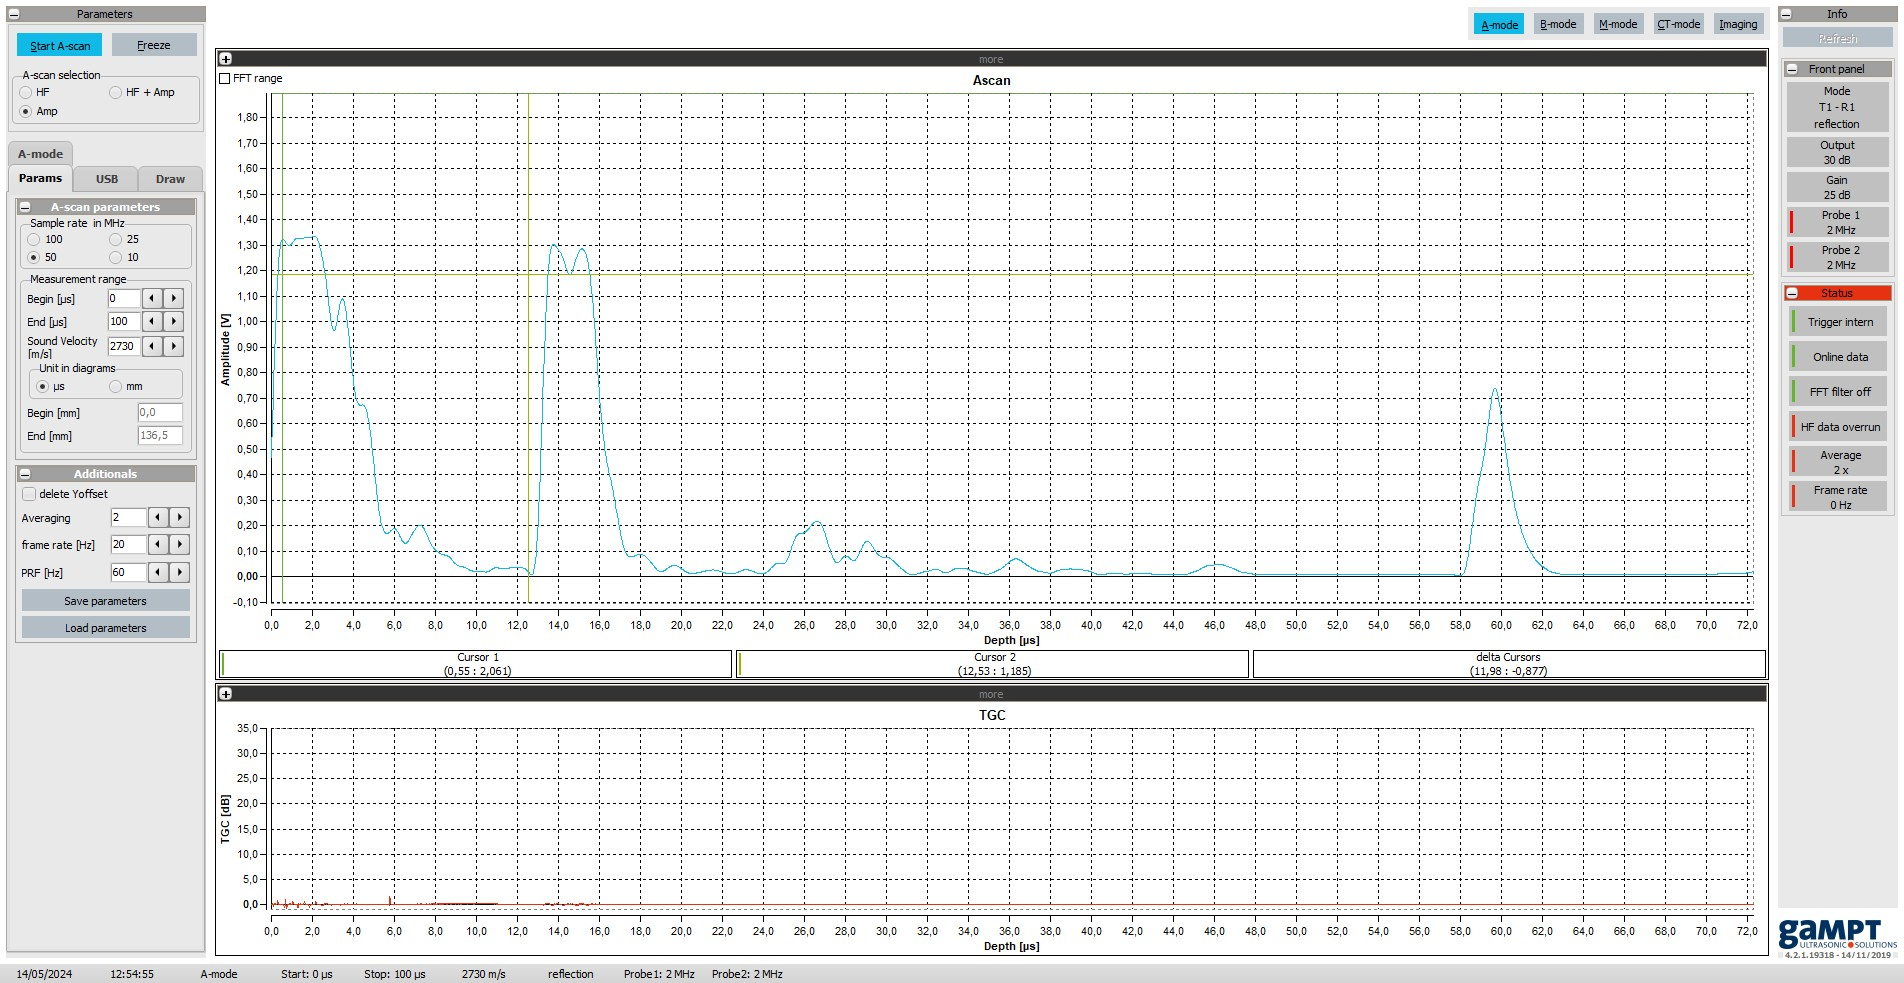
\includegraphics[height=6cm]{US2_Loch_1_2_top.jpg}
    \caption{A-Scan bei Loch 1 und 2.}
    \label{fig:Loch12}
\end{figure}

\begin{figure}[H]
    \centering 
    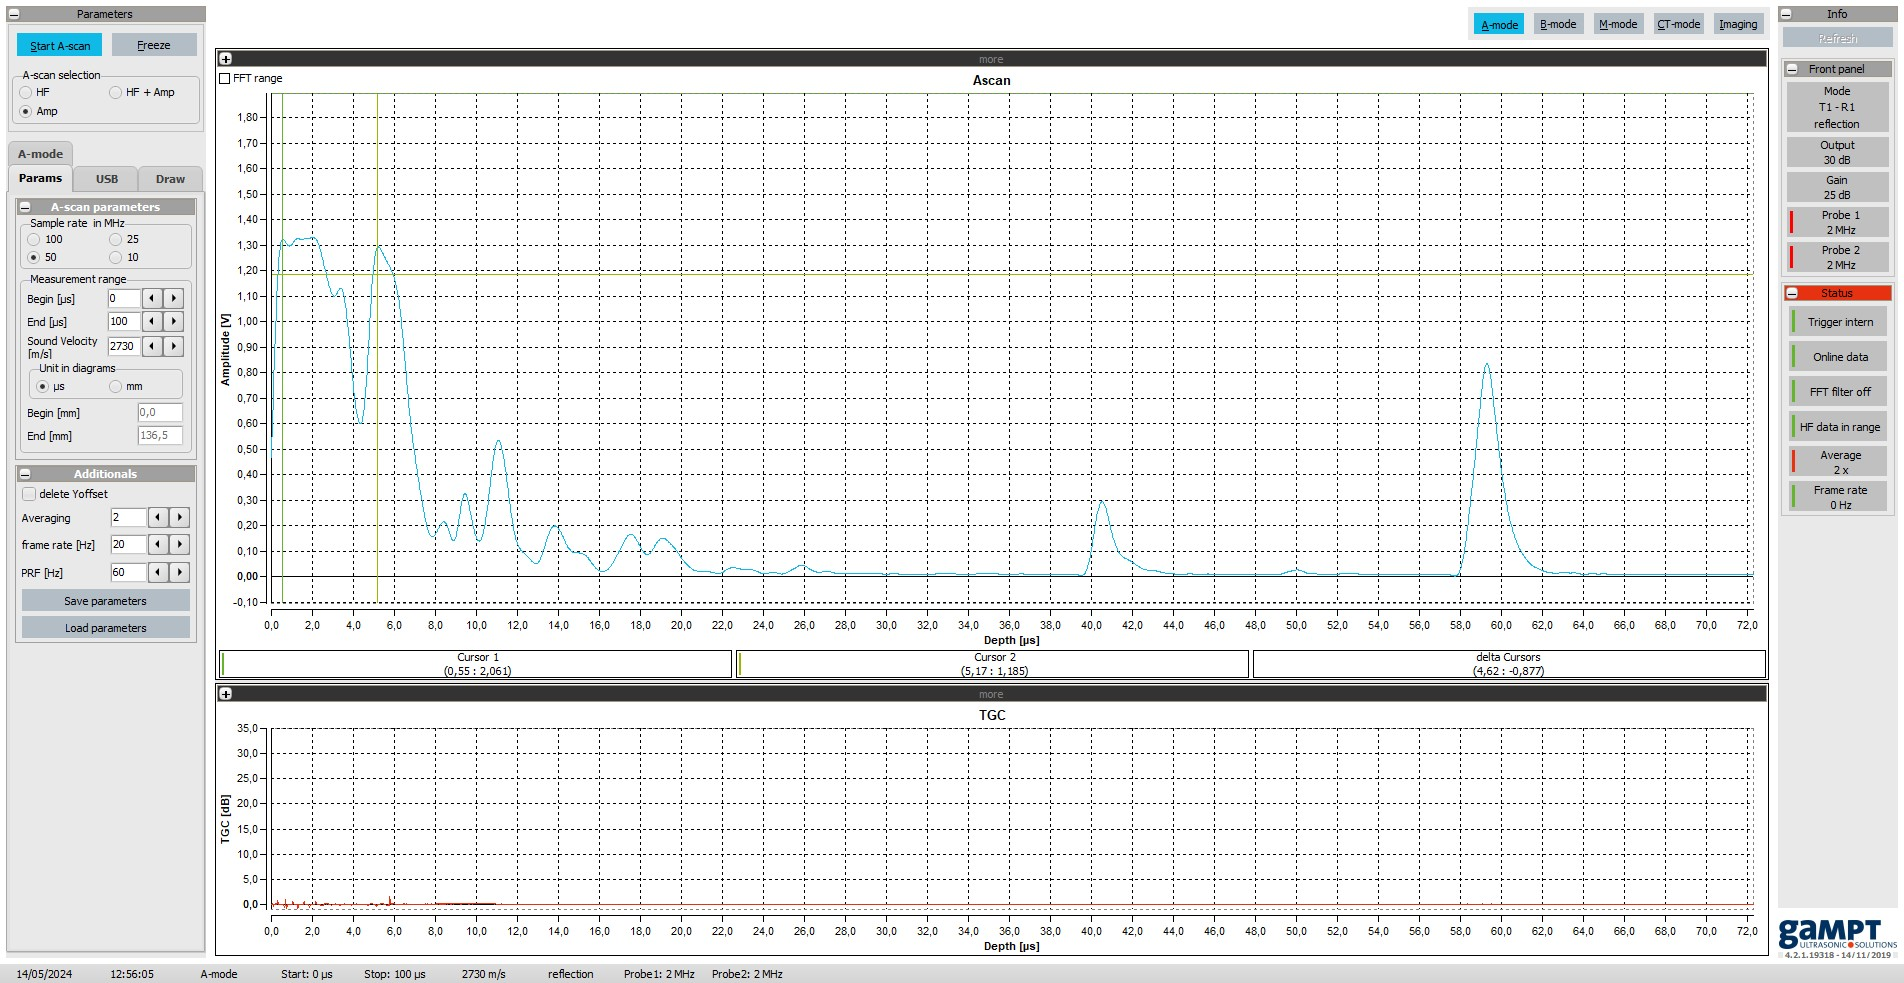
\includegraphics[height=6cm]{US2_Loch_10_top.jpg}
    \caption{A-Scan bei Loch 10.}
    \label{fig:Loch10}
\end{figure}

\noindent Im nächsten Schritt der Auswertung wird das Augenmodell mit der Intention untersucht, diverse Abstände im Auge selbst durch 
das Impuls-Echo Verfahren bestimmen zu können. Orientiert an Abb \ref{fig:Augenmodell} werden dementsprechend die Laufzeiten zur Iris, 
zu den beiden Grenzflächen der Linse und zur Retina aufgenommen:

\begin{align*}
%\label{eqn:Augenzeit}
    t_\text{Iris} &= \qty{10.66}{\micro\second}    \\ 
    t_\text{Linse,1} &= \qty{16.12}{\micro\second} \\
    t_\text{Linse,2} &= \qty{24.46}{\micro\second} \\
    t_\text{Linse,2} &= \qty{69.28}{\micro\second} \\
\end{align*}

\noindent Nach Abzug der vorhin bestimmten Anpassungszeit $t_\text{Anp}$ können nun die Distanzen durch Multiplikation mit der 
Schallgeschwindigkeit bestimmt werden. Hierbei gilt es jedoch zu beachten, dass nur die Hälfte der Laufzeiten benötigt und sich 
die Schallgeschwindigkeit aufgrund verschiedner Medien ändert! In der Glaskörperflüssigkeit beträgt die Geschwindikeit $c_\text{GK}=
\qty{1410}{\meter\second}$ und in der Linse $c_\text{L} = \qty{2500}{\meter\second}$. Daraus ergeben sich die folgenden Strecken:


\begin{align*}
%\label{eqn:Augenzeit}
    s_\text{Iris} &= \qty{7.5153}{\milli\meter}     \\
    s_\text{Linse,1} &= \qty{11.3646}{\milli\meter} \\
    s_\text{Linse,2} &= \qty{21.7896}{\milli\meter} \\
    s_\text{Linse,2} &= \qty{53.3877}{\milli\meter} \\
\end{align*}

\noindent Eine weitere medizinische Anwendungstechnik von Ultraschall besteht in der Positionsbestimmung von Tumoren. Am vorliegenden 
Brustmodell können zwei Tumore ertastet werden:

\begin{figure}
    \centering
    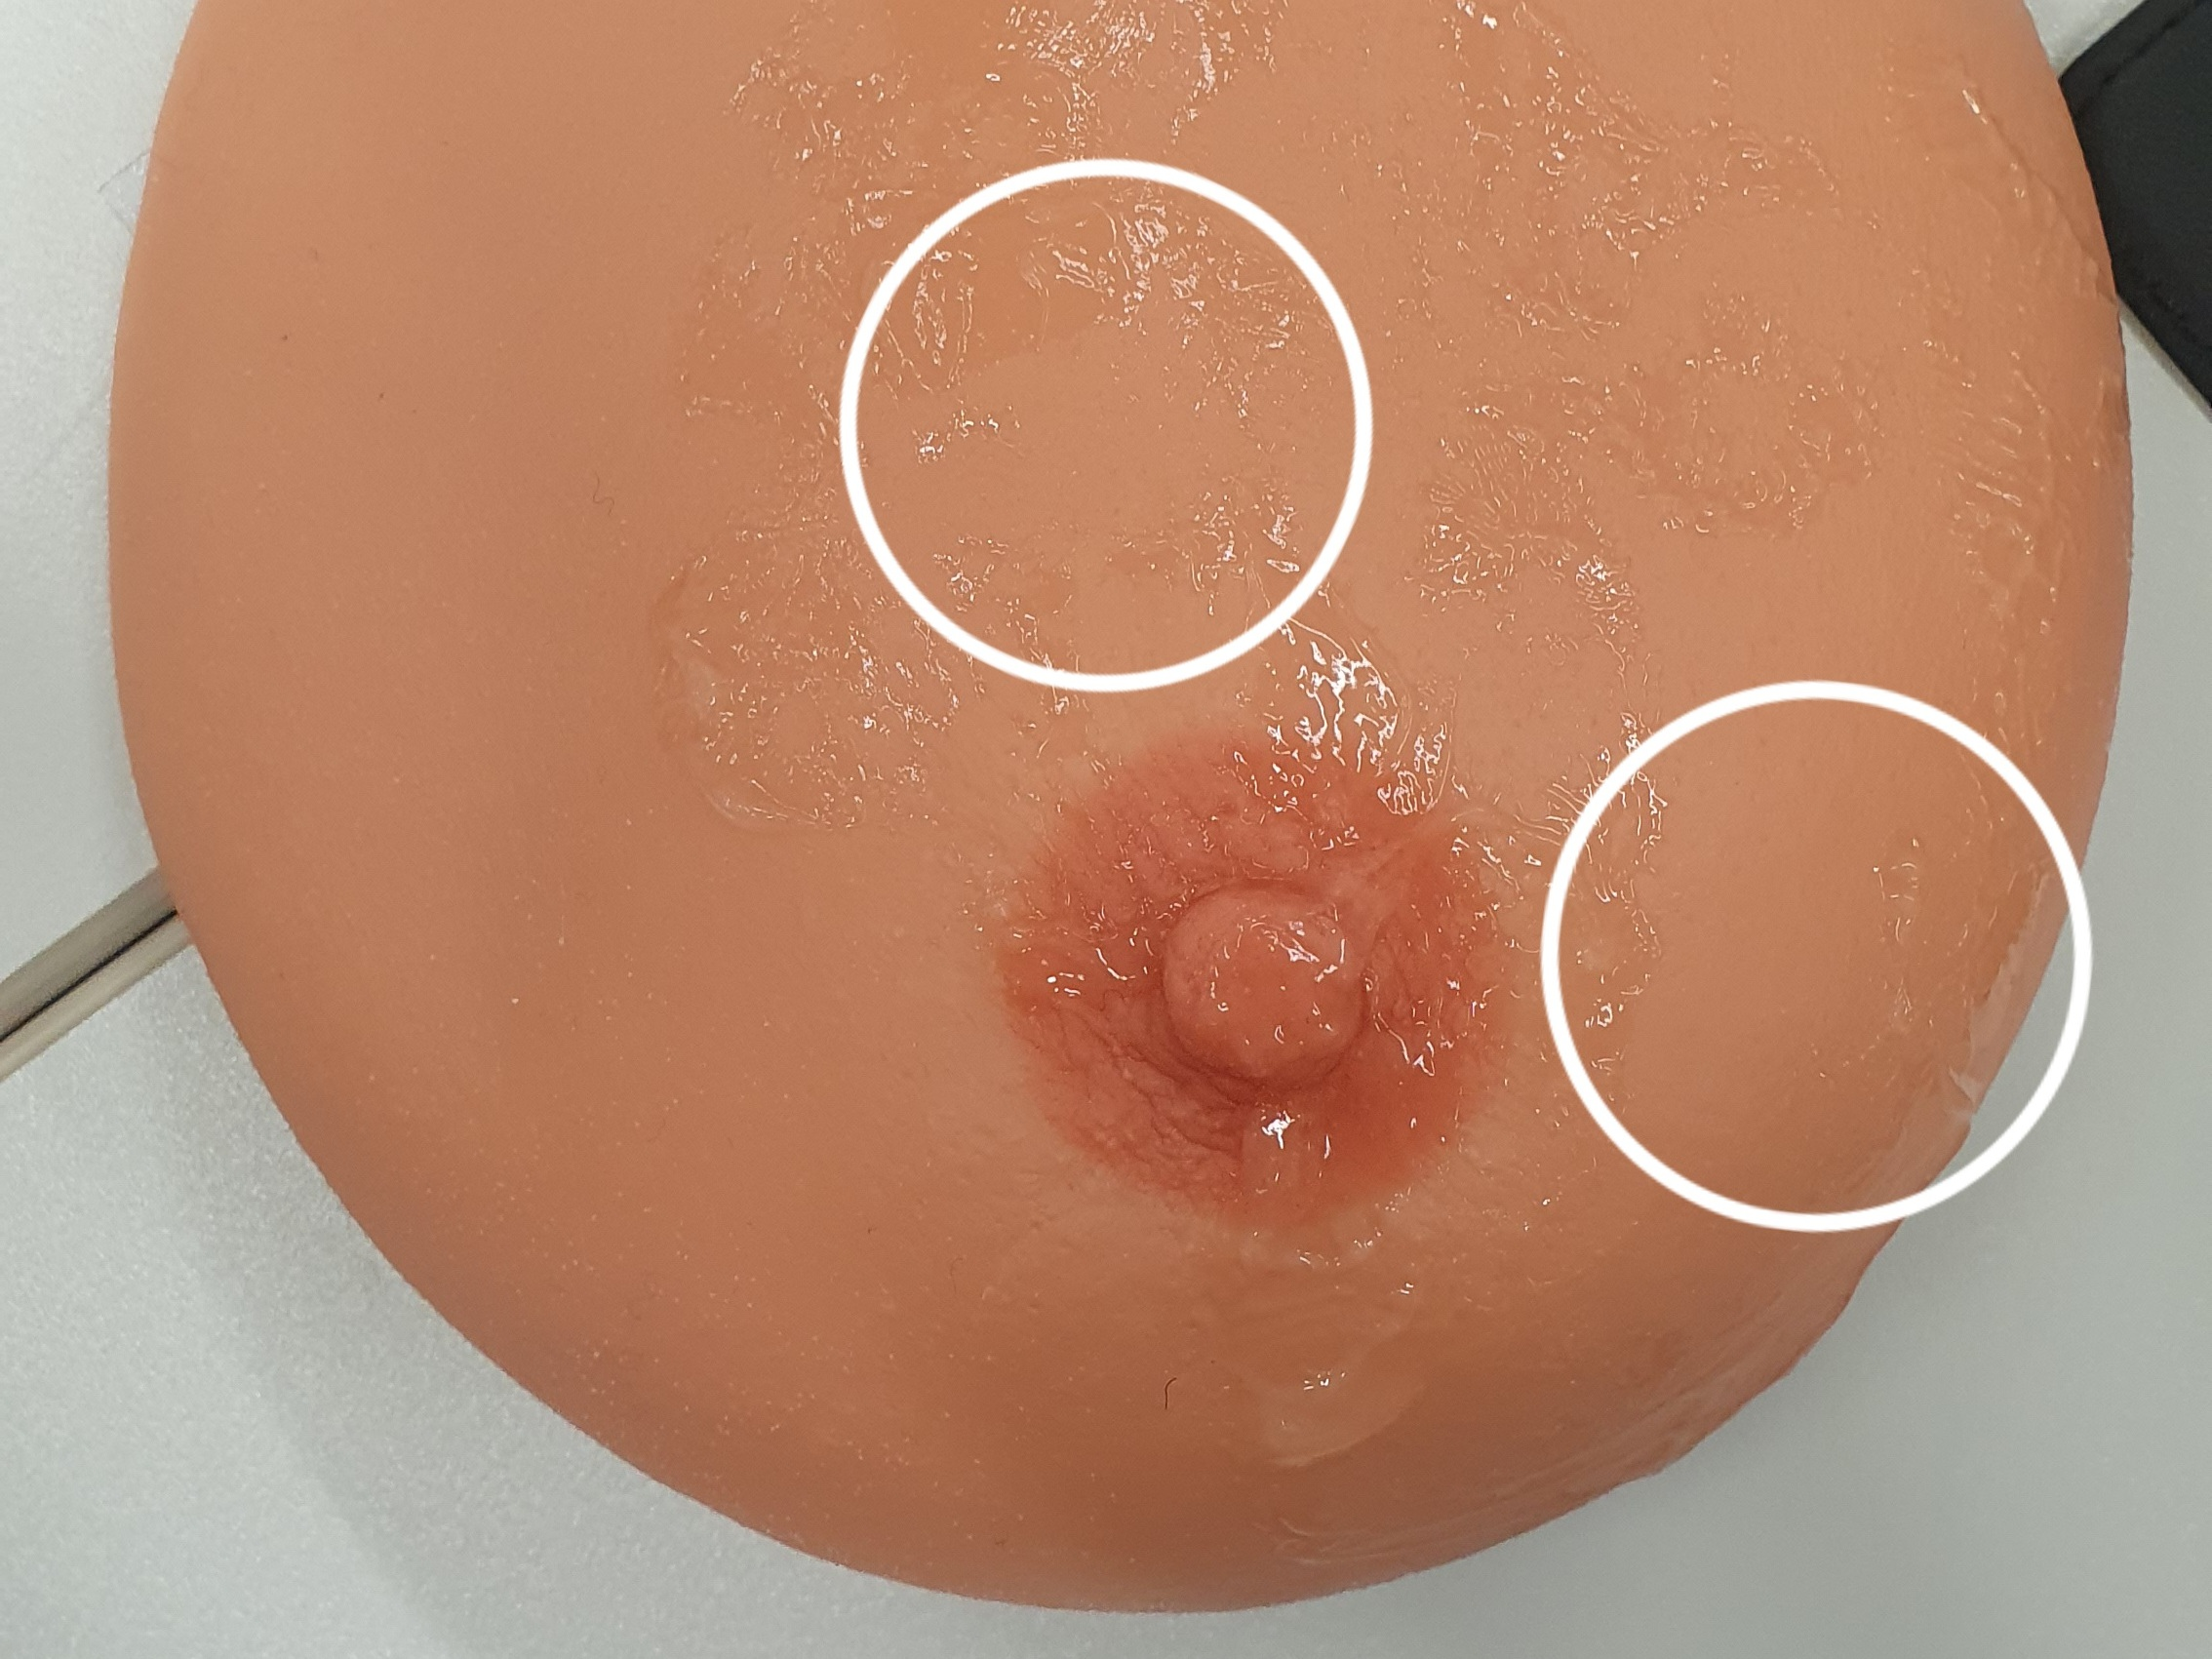
\includegraphics[height=5cm]{Tumororientierung2.jpg}
    \caption{Tumorertastung am Brustmodell.}
    \label{fig:Brust}
\end{figure}

\noindent Wie im Kapitel \ref{sec:Durchfuehrung} beschrieben, wird mittels einer beweglichen \qty{2}{\mega\hertz} Sonde ein 
\emph{B-Scan} aufgenommen. Dieser liefert für die in der Abbildung \ref{fig:Brust} erkennbaren Tumore das folgende Bild:

\begin{figure}
    \begin{subfigure}{0.48\textwidth}
        \centering
        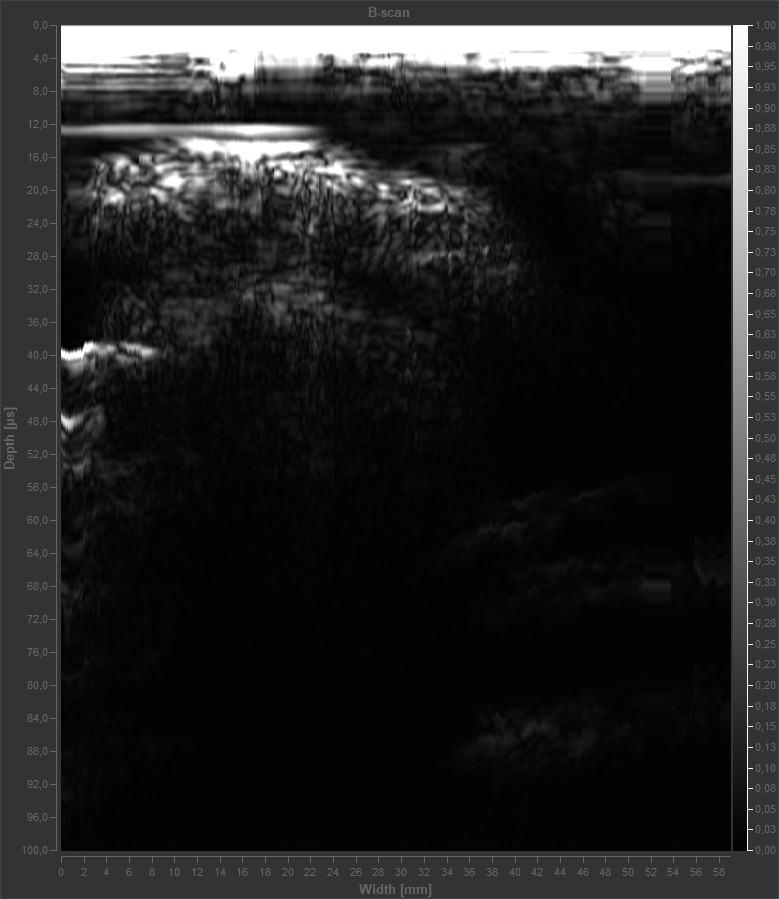
\includegraphics[height=6cm]{Tumor_rechts_2.jpg}
        \caption{Tumor rechts.}
        \label{fig:TR}
    \end{subfigure}
    \hfill
    \begin{subfigure}{0.48\textwidth}
        \centering 
        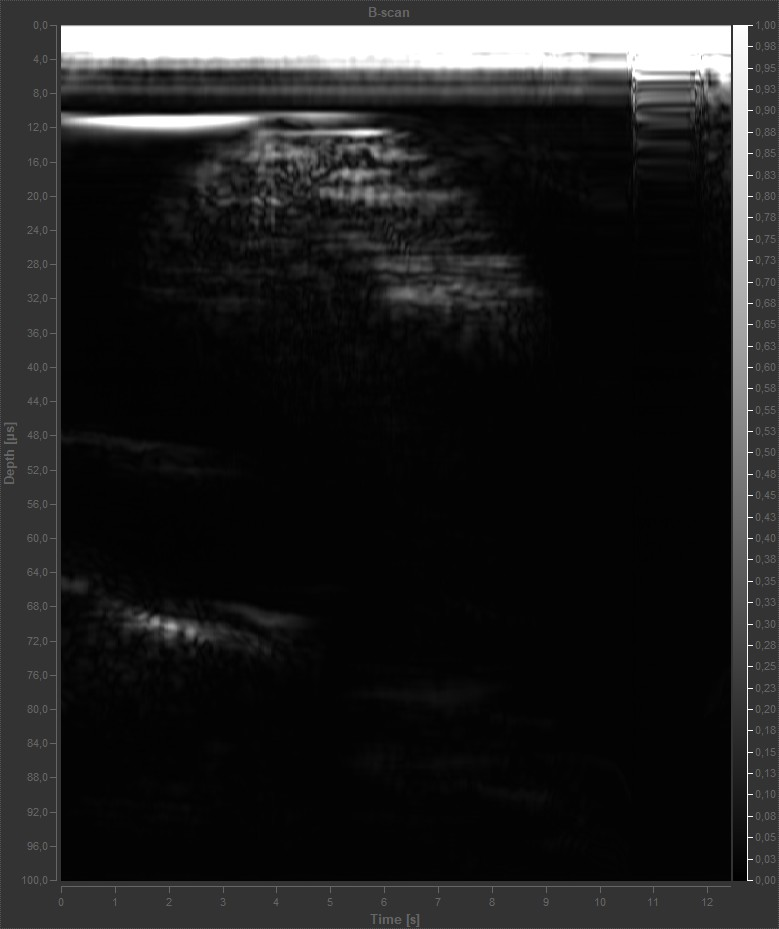
\includegraphics[height=6cm]{Tumor_oben.jpg}
        \caption{Tumor oben.}
        \label{fig:TO}
    \end{subfigure}
    \caption{Tumorpositionierung im Brustmodell.}
    \label{fig:Vergleich}
\end{figure}

\noindent XXX\\

\noindent Im letzten Part des Experiments soll das Herzzeitvolumen $\left(HZV\right)$ bestimmt werden. Hierfür benötigen wir demnach 
die Werte für das endsystolische Volumen $\left(ESV\right)$ und die Periodendauer $T$. Folgende Messungen werden notiert:

\begin{table}[H]
    \centering 
    \caption{Untersuchung eines Herzmodells mit dem \emph{TM-Scan}.}
    \label{tab:Herzmodell}
    \begin{tblr}{
        colspec = {S[table-format=1.2] S[table-format=2.2]},
        row{1} = {guard, mode=math},
        }
        \toprule 
        \text{Periodendauer } T \mathbin{/} \unit{\second} & \text{Auslenkung} \mathbin{/} \unit{\micro\second} \\
        \midrule 
        2.17  &  12.24 \\
        2.25  &  10.30 \\
        1.73  &  10.30 \\
        1.73  &  10.30 \\
        1.66  &  10.78 \\
        1.79  &  11.26 \\
        1.50  &  11.26 \\
        1.73  &  11.26 \\
        1.47  &  10.90 \\
        \bottomrule 
    \end{tblr}
\end{table}

\noindent Aus dem Mittelwert der Periodendauern lässt sich die Herzfrequenz $f_\text{Herz}$ berechnen. Zusätzlich wird das 
endsystolische Volumen als Kegel mit Durchmesser $d = \qty{45.5\pm0.025}{\milli\meter}$ und Höhe $h$, welche dem Mittelwert
der Auslenkunge aus \ref{tab:Herzmodell} entspricht, approximiert. Nach dieser Rechnung beträgt das Herzzeitvolumen 

\begin{equation*}
    HZV = \qty{3.334\pm0.004}{\cubic\milli\meter}
\end{equation*}
\end{document}
